When describing rotating particles it is common to use the so called Euler Angles. A formal definition can be found at MathWorld \cite{eulerAngles} but for the purposes of this thesis we will describe it as a transformation from a coordinate system $\{x,y,z\}$ to \{x',y',z'\} in three steps

\begin{itemize}
\item Rotate the x-y plane $\phi$ about the z-axis.
\item Denote the shifted x axis T and rotate the z-y' plane $\theta$ around this axis
\item Rotate $\psi$ around the z' axis to obtain the final coordinate system
\end{itemize}

This is illustrated in figure \ref{fig:eulerangles} where each prim marks one more step of rotation to the coordinate system. To make it clear how this relates to the experiment figure \ref{fig:eulerparticle} shows the euler angle rotations for a triaxial particle shown from a point of view similar to the of the experiment where the X-Z plane is the primary plane. 

\begin{figure}
\begin{center}
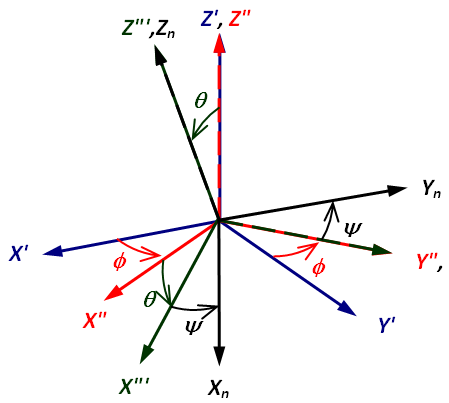
\includegraphics[width=0.7\textwidth]{figures/theory/eulerangles.png}
\end{center}
\caption{The Euler angles illustrated using a series of coordinate rotations. This is the normal way of illustrating the Euler angles as it is how they are defined.}
\label{fig:eulerangles}
\end{figure}


\begin{figure}
\begin{center}
\includegraphics[width=0.6\textwidth]{figures/theory/EulerParticle.pdf}
\end{center}
\caption{The Euler angles illustrated using an ellipsoid. This alternate visualization shows the angles with a point of view similar to that of the camera in the experiment. Note although $\psi$ has an impact on the particle dynamics, as the particle is nearly axis-symmetric we can not observe it}
\label{fig:eulerparticle}
\end{figure}

% Write something about the coordinate system here